\documentclass[]{article}

\usepackage[utf8]{inputenc}  %codage du fichier source pour avoir les
% accents français
\usepackage[T1]{fontenc}  %codage des fontes TEX
\usepackage[french]{babel}  %document en français
% Pour les guillemets français « = Alt Gr + Z   et » = Alt Gr + X
\RequirePackage{fancyhdr} % pour les en-tetes et pieds de pages
\usepackage{graphicx} % Pour les figures
\RequirePackage{vmargin} %Pour modifier les marges
\RequirePackage{lastpage}  % Pour le numéro de la dernière page
\usepackage{amsmath} % Pour des accessoires en environnement math
\usepackage{array}
\usepackage{enumerate}


\begin{document}
\pagestyle{empty} 
\setpapersize{A4}

\section{Résolution directe avec différents schémas}

Pour cette comparaison des différents schéma d'intégration pour le résolution
directe du problème de dynamique, nous avons choisi d'implémenter 3 schémas
d'intégration: le schéma implicite d'Euler à un pas, le schéma explicite des
différence centrées et le schéma de Newmark plus général (en effet le schéma
des différences centrées est un schéma de Newmark).

\subsection{Le schéma implicite d'Euler}

Nous avons choisi d'implémenter le schéma implicite d'Euler à un pas or
l'équation de la dynamique est $\underline{\underline{M}}\underline{\ddot{X}} +
\underline{\underline{K}}\underline{X} = \underline{F}(t)$ donc pour utiliser
un schéma à un pas ce système doit être modifier. Pour cela, on introduit un
vecteur $\underline{Q}$ tel que:
\begin{displaymath}
% use packages: array
\underline{Q}=
\left\lbrace  \begin{array}{c}
\underline{X} \\ 
\underline{\dot{X}}
\end{array}\right\rbrace 
\end{displaymath}
Ce qui conduit au système suivant, du premier ordre par rapport à
$\underline{Q}$:
\begin{displaymath}
\left( \begin{array}{cc}
\underline{\underline{Id}} & 0 \\ 
0 & \underline{\underline{M}}
\end{array}\right) 
\left\lbrace  \begin{array}{c}
\underline{\dot{X}} \\ 
\underline{\ddot{X}}
\end{array}\right\rbrace  +
\left( \begin{array}{cc}
0 & -\underline{\underline{Id}} \\ 
\underline{\underline{K}} & 0
\end{array}\right)
\left\lbrace  \begin{array}{c}
\underline{X} \\ 
\underline{\dot{X}}
\end{array}\right\rbrace  = 
\left\lbrace \begin{array}{c}
0 \\ 
\underline{F}(t)
\end{array}\right\rbrace 
\end{displaymath}
On écrit ensuite le schéma implicite d'euler de la façon suivante:
$$
\underline{\dot{Q}}_{n+1} = \dfrac{\underline{Q}_{n+1} -
\underline{Q}_{n}}{\Delta t}
$$
On peut donc obtenir l'expression de $\underline{Q}_{n+1}$ en fonction de
$\underline{Q}_{n}$:
$$
\underline{\underline{\tilde{M}}}\cdot\underline{\dot{Q}}_{n+1} +
\underline{\underline{\tilde{K}}}\cdot\underline{Q}_{n+1} =
\underline{\tilde{F}}$$
$$\Rightarrow \underline{Q}_{n+1} = \left( \underline{\underline{\tilde{M}}} +
\Delta t \underline{\underline{\tilde{K}}}\right)^{-1}\cdot\left( \Delta t
\underline{\tilde{F}} + \underline{Q}_{n}\right) $$
Grâce à cette expression, il est possible de résoudre l'equation de la
dynamique. Ce schéma est particulièrement intéressant car il est
inconditionnelement stable.

\paragraph{Résultats:}~\\

Les résultats de la Figure~\ref{defimp} ont été obtenu pour le schéma implicite
d'euler pour $\Delta t=0.01\ s$ avec une poutre de longueur $L=500\ m$ (afin de
pouvoir observer les reflexions) avec 160 éléments dans la longueur. L'effort
$F=10000\ N$ est appliqué entre t=0.2s et t=0.4s, sur une durée de calcul de 2s.

\begin{figure}
\begin{center}
 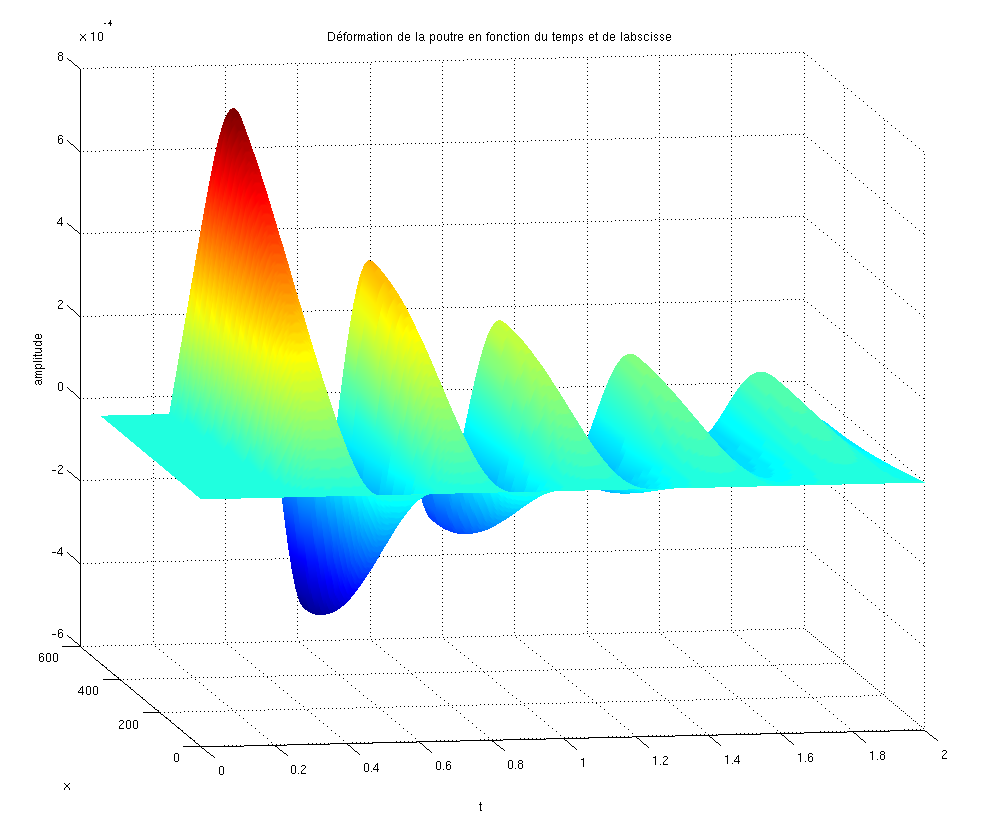
\includegraphics[scale=0.2]{Figures/3D_def.png}
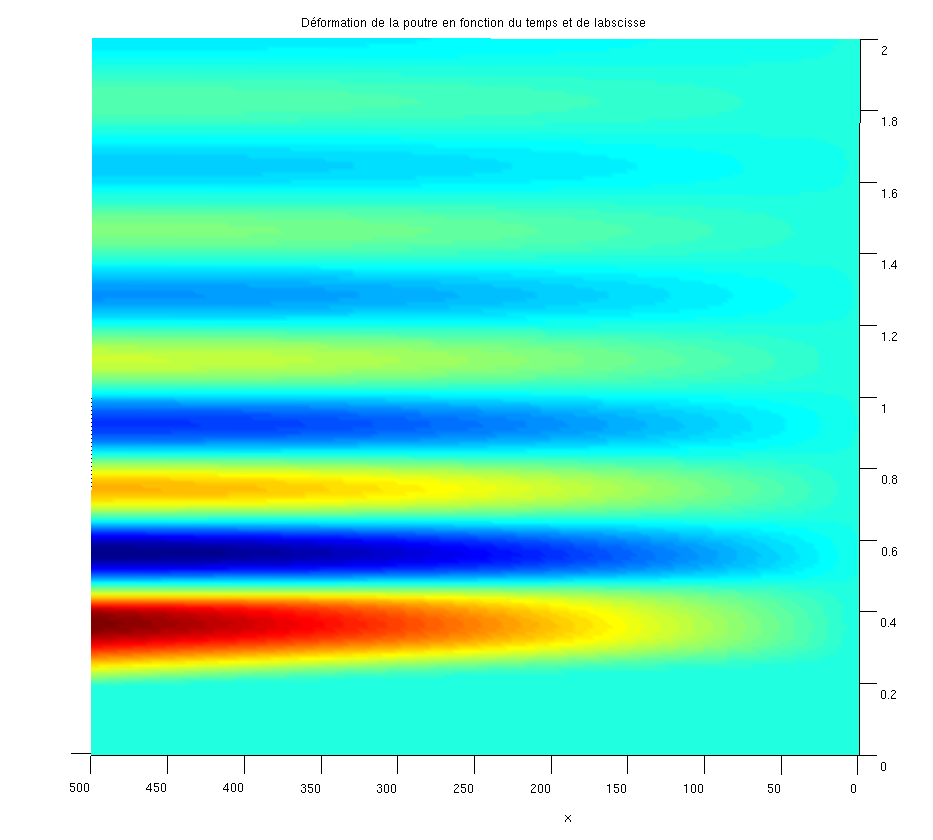
\includegraphics[scale=0.2]{Figures/3D_def_2.png}
\caption{Déformation de la poutre en fonction du temps et de l'espace}
\label{defimp}
\end{center}
\end{figure}

Les rélexions de l'onde au niveau des extrémités de la poutre sont bien visibles
sur la Figure~\ref{defimp}. Il est également possible de voir que l'amplitude
des réflexions diminue au cours du temps. Cette constation est confirmée par la
Figure~\ref{enerimp} qui représente l'energie totale du système en fonction du
temps (Energie cinétique + energie de déformation). Cette énergie diminue au
cours du temps, alors que l'on s'attend à ce que cette énergie soit constante
pour t>0.4s car notre système n'est pas un système dissipatif, en effet nous
avons négligé l'amortissement dans l'équation de la dynamique. Cette diminution
de l'énergie totale du système est un problème bien connue du schéma d'Euler
implicite. Pour diminuer ces effet de dissipation du schéma numérique, il faut
diminuer $\Delta t$. La Figure~\ref{enerimp} permet d'illustrer cela, en effet
le graphique de droite provient du calcul avec $\Delta t = 0.01\ s$ présente
une attenuation de l'énergie plus importante que le graphique de droite
provenant du calcul avec $\Delta t=0.005\ s$. Mais la diminution de $\Delta t$
va entrainer une augmentation du temps de calcul. La Figure~\ref{analimp}
permet de voir que l'augmentation du temps de calcul croit beaucoup plus vite
que l'erreur relative sur la valeur finale de l'energie totale ne diminue. Ce
qui veut donc dire que pour avoir une attenuation faible il va falloir avoir un
$\Delta t$ vraiment très petit et donc un temps de calcul trop important. On
voit donc apparaître ici une des limites du schéma implicite d'Euler à un pas.
\begin{figure}
\begin{center}
 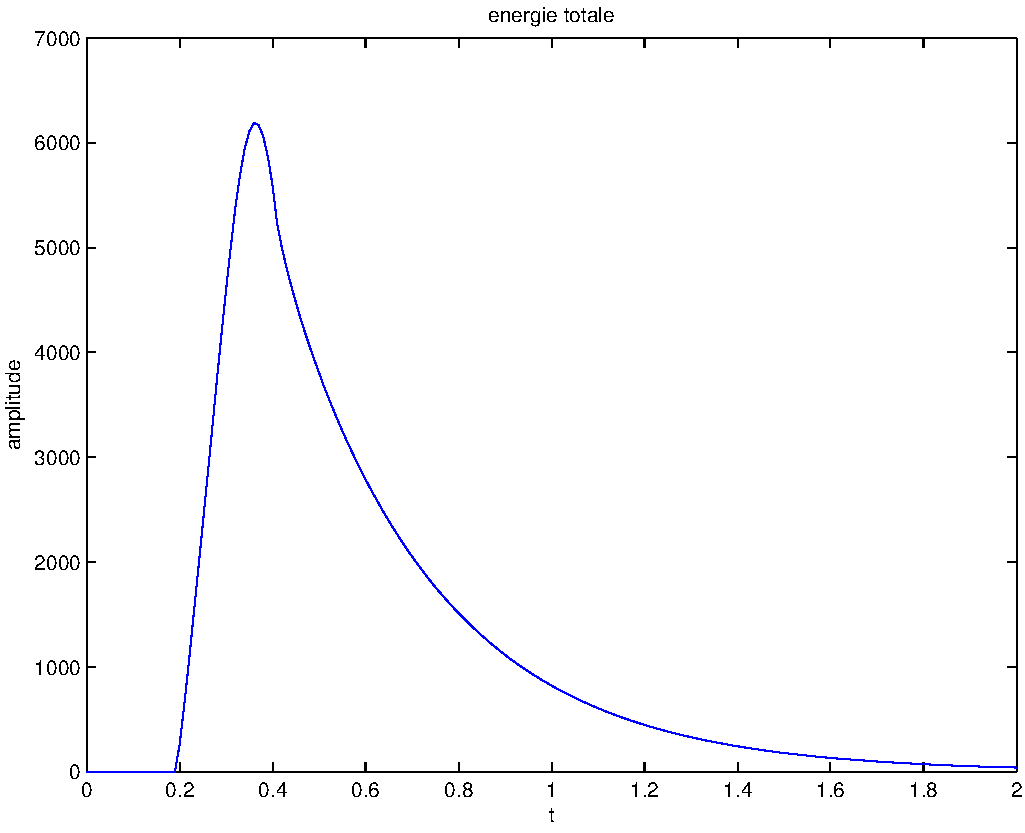
\includegraphics[scale=0.4]{Figures/fig3_mod.pdf}
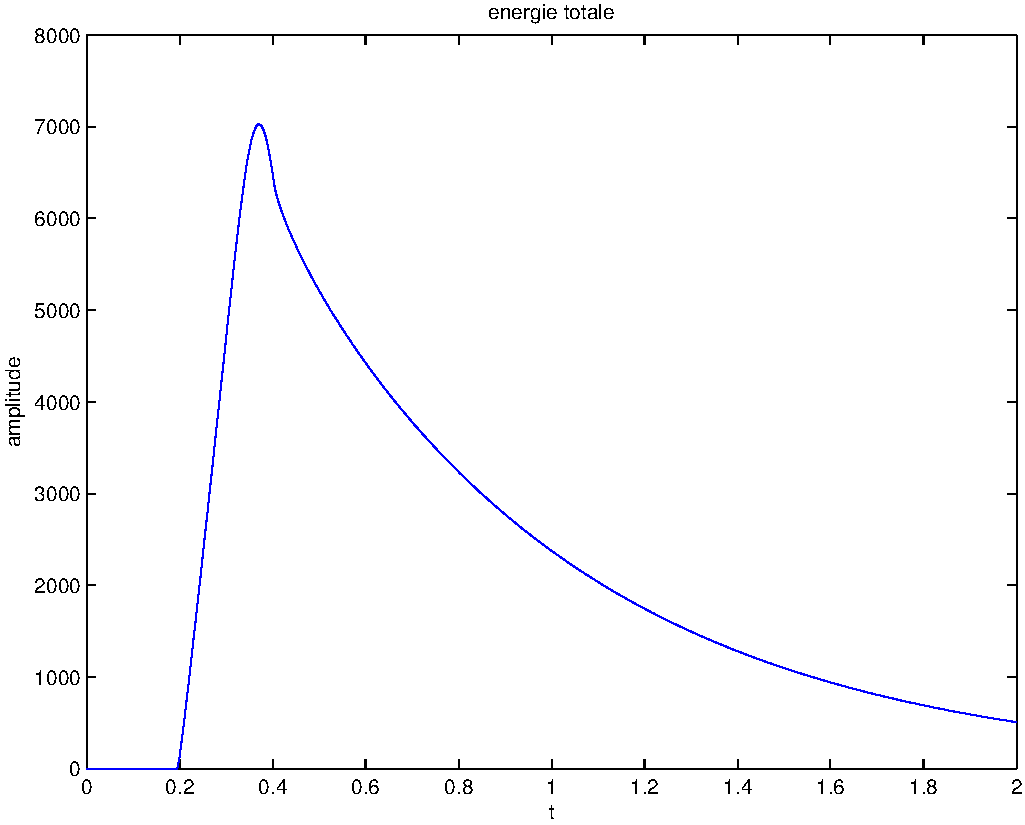
\includegraphics[scale=0.4]{Figures/fig3_mod2.pdf}
\caption{Evolution de l'énergie totale du système en fonction du temps (à
gauche pour $\Delta t=0.01\ s$ et à droite pour $\Delta t=0.005\ s$}
\label{enerimp}
\end{center}
\end{figure}

\begin{figure}
\begin{center}
 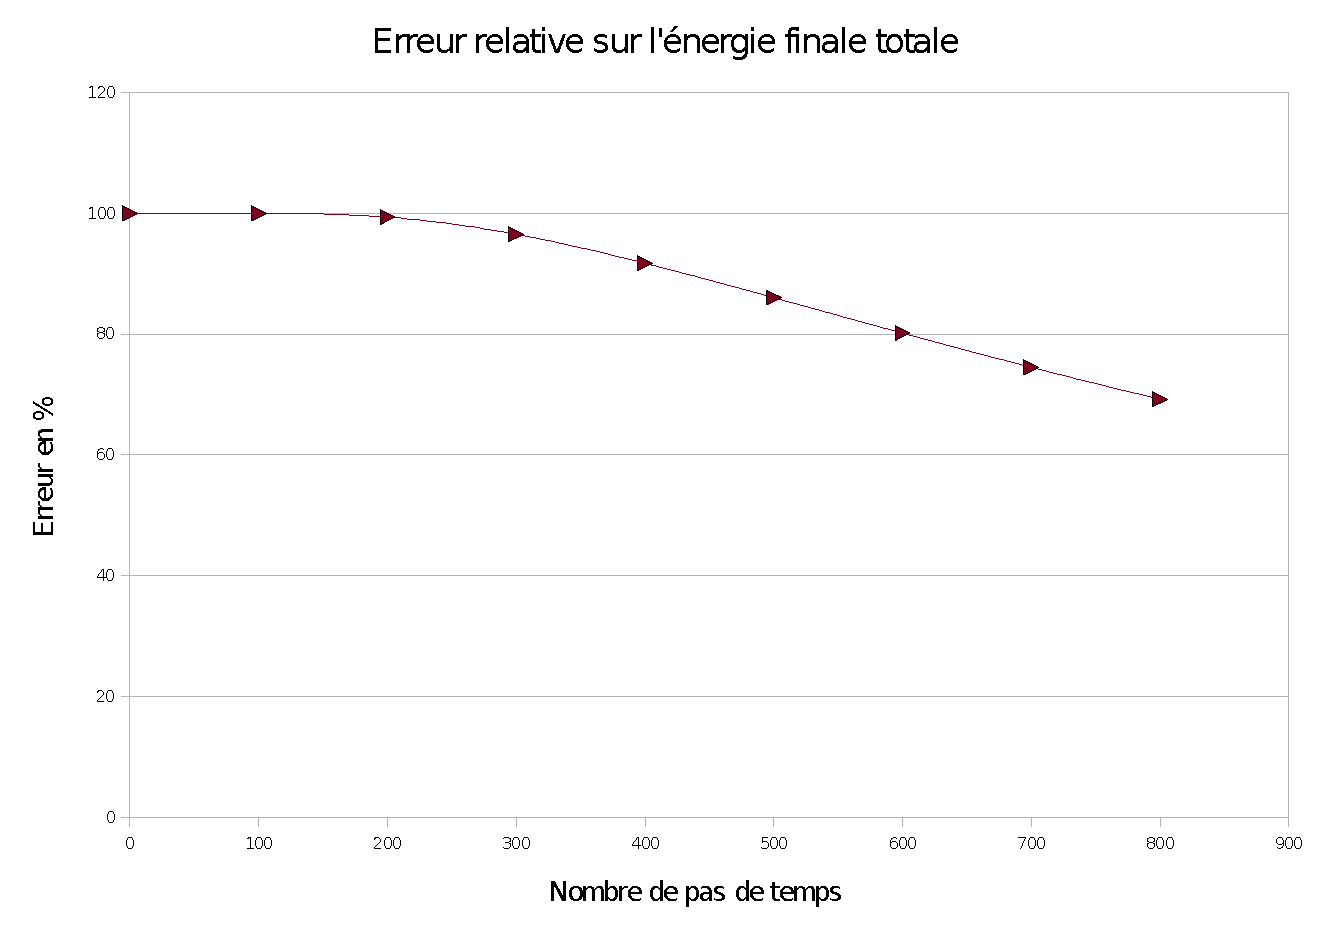
\includegraphics[scale=0.32]{Figures/Erreur.pdf}
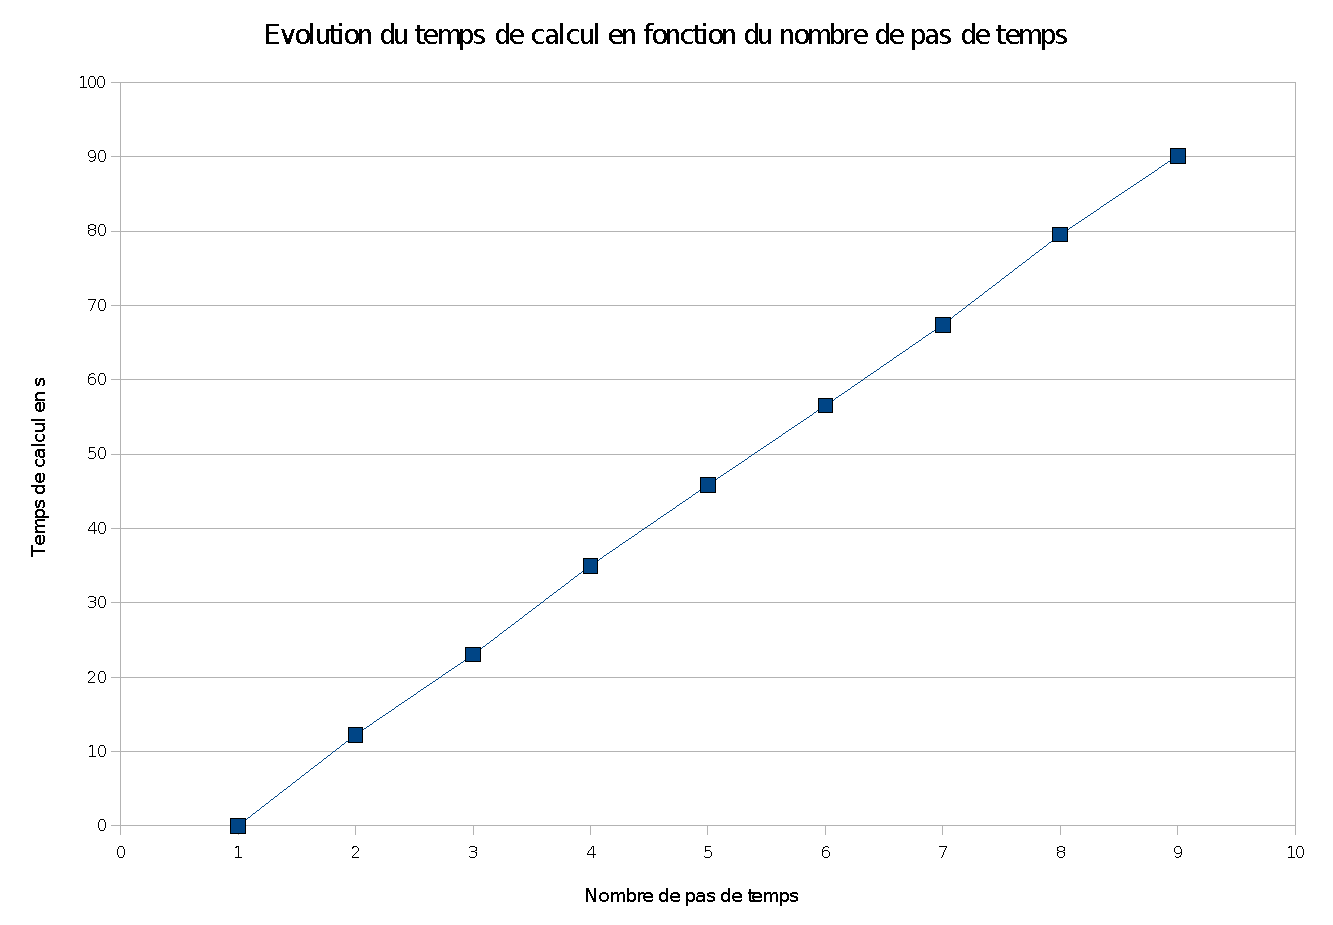
\includegraphics[scale=0.32]{Figures/temps.pdf}
\caption{Evolution du temps de calcul (à gauche) et de l'erreur relative
 sur la valeur de l'énerge totale finale (à droite) en fonction du nombre de
pas de temps}
\label{analimp}
\end{center}
\end{figure}

\subsection{Schéma explicite des différences centrées}

Le principe de ce schéma est le suivant:
\[
\left \{
\begin{array}{c @{=} c}
    \dot{x}_{n+\frac{1}{2}} & \frac{1}{\Delta t} ( x_{n+1} - x_{n} ) \\
    \ddot{x}_{n} & \frac{1}{\Delta t} ( \dot{x}_{n+\frac{1}{2}} -
\dot{x}_{n-\frac{1}{2}} ) \\
\end{array}
\right.
\]
Ce schéma est conditionnellement stable. En effet ce schéma est un schéma de
Newmark avec $\gamma=\frac{1}{2}$ et $\beta=0$, qui ne verifie donc pas la
condition de stabilité inconditionnelle qui est $2\beta-\gamma\geq0$. La
condition de stabilité conditionnelle pour le schéma des différences centrées
est:
$$ \Delta t \leq \Delta t_{crit}= \min_{j} \frac{2}{w_{j}}$$
A l'aide de ce qui a été précédement fait pour obtenir la base modale, il est
possible de déterminer le $\Delta t_{crit}$ et ainsi choisir une valeur de
$\Delta t$ qui assure la convergence du calcul. Il est important de noter que
dans le cadre de cette étude la détermination de $\Delta t_{crit}$ est assez
facile et peu couteuse, mais cela n'est pas le cas dans la majeure partie des
problèmes.
$$
\Delta t_{crit} = 2 / \sqrt{3.8617*10^{7}} = 3.21*10^{-4}\ s
$$
Dans notre cas, la durée de calcul est de 2s, il nous faut donc au moins 6215
pas de calcul pour s'assurer la convergence du schéma. La Figure~\ref{convdiv}
permet de vérifier ce résultat sur notre programe, les deux figures représente
nt le déplacement de l'extrémité de la poutre en fonction du temps, sur la
figure de gauche le calcul diverge alors que sur la figure de droite avec un
pas de temps en plus le calcul converge. 
\begin{figure}
\begin{center}
 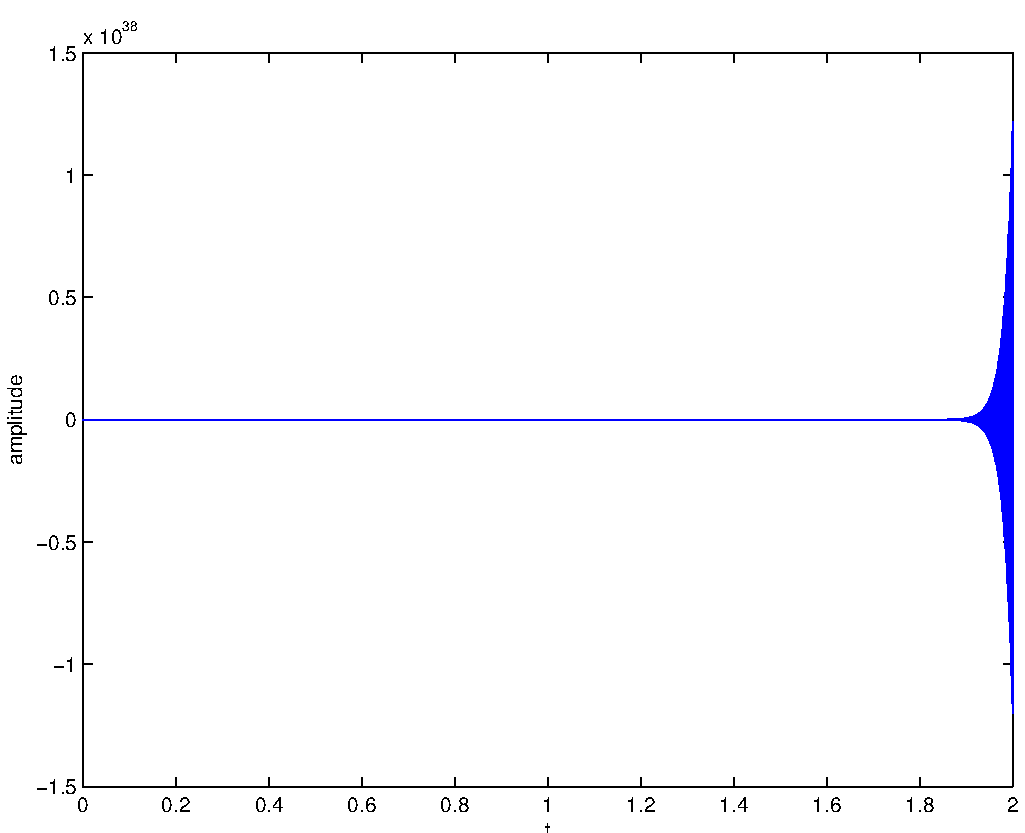
\includegraphics[scale=0.42]{Figures/depldifcendiv.pdf}
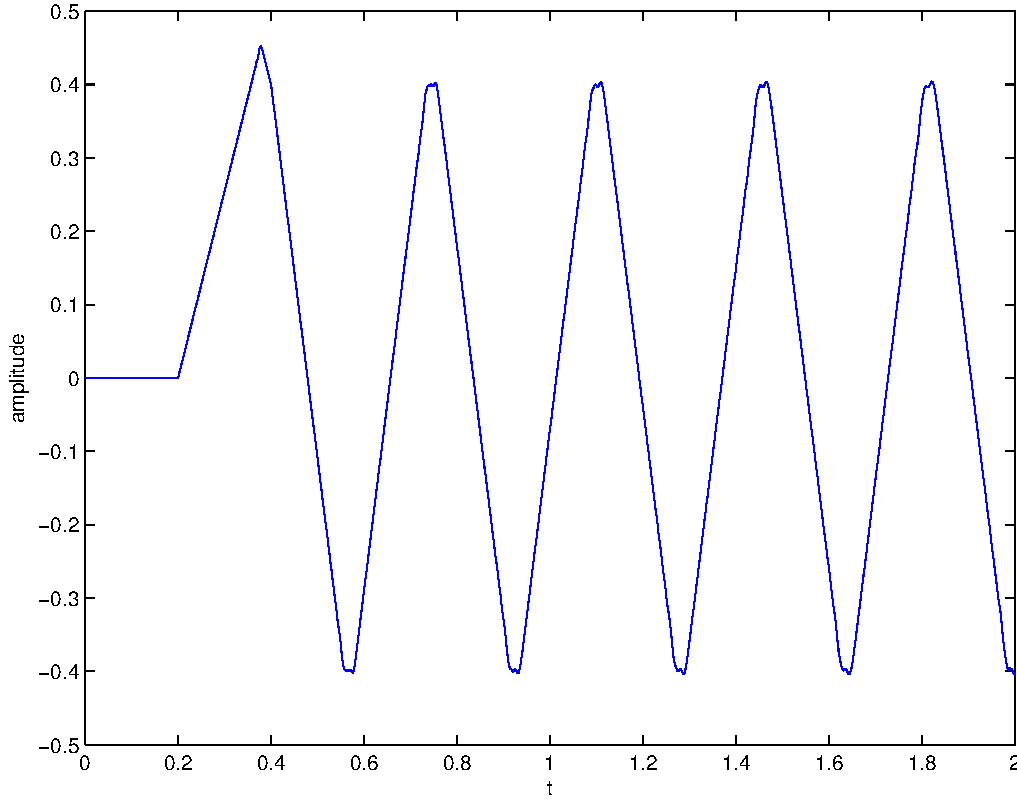
\includegraphics[scale=0.42]{Figures/depldifcenconv.pdf}
\caption{Déplacement de l'extrémité de la poutre en fonction du temps pour un
calcul avec 6214 pas de temps à gauche et 6215 à droite}
\label{convdiv}
\end{center}
\end{figure}
A la fin de cette partie, une comparaison entre ce schéma et un schéma de
Newmark optimisé va être réalisée.

\subsection{Schéma de Newmark à un pas}

\end{document}